\documentclass[12pt,a4paper,twocolumn]{article}
% The following LaTeX packages must be installed on your machine: amsmath, authblk, bm, booktabs, caption, dcolumn, fancyhdr, geometry, graphicx, hyperref, latexsym, natbib
\input{151.dat}
\usepackage{gensymb}
\usepackage{float}
\usepackage{siunitx}
\usepackage{amssymb}
\usepackage{float}
\usepackage{enumerate}
\usepackage{listings}
\PassOptionsToPackage{hyphens}{url}\usepackage{hyperref}
\usepackage[none]{hyphenat}
%\renewcommand{\familydefault}{\sfdefault}


\begin{document}

\setcounter{page}{1}

\section*{Problem 2.13}
\bigskip

\begin{figure}[htb]
	\centering
	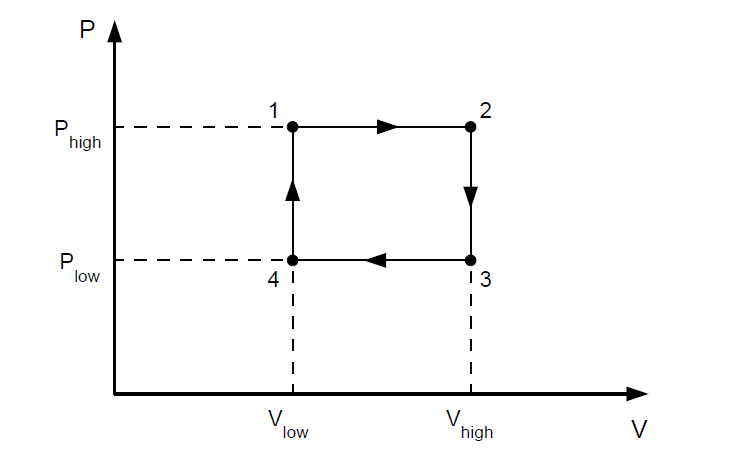
\includegraphics[width=0.45\textwidth]{work.png}
	\caption{Cyclic process for this problem.}
	\label{fig:cycle}
\end{figure}

From Example 2.1, the net work done on a gas in a cyclic process was determined to be nonzero, with a value of

\begin{equation}\label{oldanswer}
	W_{net} = -\left( P_{high} - P_{low} \right) \left( V_{high} - V_{low} \right)
\end{equation}

Assuming an ideal gas with $N$ particles, the energy transfer due to heating for each step in the process is as follows:

\begin{align}
	Q_{1 \rightarrow 2} = -Q_{3 \rightarrow 4} & = \int_{T_1}^{T_2} c_P \textrm{ d}T \\
	& = \nu c_P \int_{T_1}^{T_2} \textrm{ d}T \\
	& = \nu c_P \left( T_2 - T_1 \right) \\
	& = \nu c_P \Delta T \label{eq:isobaric} \\
	Q_{2 \rightarrow 3} = -Q_{4 \rightarrow 1} & = \int_{T_1}^{T_2} c_V \textrm{ d}T \\
	& = \nu c_V \int_{T_1}^{T_2} \textrm{ d}T \\
	& = \nu c_V \left( T_2 - T_1 \right) \\
	& = \nu c_V \Delta T \label{eq:isochoric}
\end{align}

Recalling the ideal gas equation,

\begin{eqnarray}
	PV = \nu RT \label{eq:idealgas} \\
	T = \frac{PV}{\nu R} \label{eq:idealtemp}
\end{eqnarray}

The net energy transfer due to heating is

\begin{equation}\label{eq:totalwork}
	W_{net} = Q_{1 \rightarrow 2} + Q_{2 \rightarrow 3} + Q_{3 \rightarrow 4} + Q_{4 \rightarrow 1}
\end{equation}

Plugging \eqref{eq:idealtemp} into each of the equations in \eqref{eq:isobaric} and \eqref{eq:isochoric}, we have

\begin{align}
	Q_{1 \rightarrow 2} & = \nu c_P P_{high} \frac{V_{high} - V_{low}}{\nu R} \label{eq:Q12plug} \\
	Q_{2 \rightarrow 3} & = \nu c_V V_{high} \frac{P_{low} - P_{high}}{\nu R} \label{eq:Q23plug} \\
	Q_{3 \rightarrow 4} & = \nu c_P P_{low} \frac{V_{low} - V_{high}}{\nu R} \label{eq:Q34plug} \\
	Q_{4 \rightarrow 1} & = \nu c_V V_{low} \frac{P_{high} - P_{low}}{\nu R} \label{eq:Q41plug}
\end{align}

Simplifying equations \eqref{eq:Q12plug} through \eqref{eq:Q41plug} and summing them as in \eqref{eq:totalwork}, we have

\begin{align}
	Q_{net} & = c_P P_{high} \frac{V_{high} - V_{low}}{R} \nonumber \\
	& - c_V V_{high} \frac{P_{high} - P_{low}}{R} \nonumber \\
	& - c_P P_{low} \frac{V_{high} - V_{low}}{R} \nonumber \\
	& + c_V V_{low} \frac{P_{high} - P_{low}}{R}
\end{align}
\begin{align}
	Q_{net} & = \frac{c_P}{R} \left( P_{high} - P_{low} \right) \left( V_{high} - V_{low} \right) \nonumber \\
	& -\frac{c_V}{R} \left( P_{high} - P_{low} \right) \left( V_{high} - V_{low} \right) \label{eq:Wnetplug}
\end{align}

Recall that for an ideal gas,

\begin{eqnarray}
	c_P = \frac{5}{2} R \label{eq:idealcp} \\
	c_V = \frac{3}{2} R \label{eq:idealcv}
\end{eqnarray}

Plugging these into \eqref{eq:Wnetplug},

\begin{align}
	Q_{net} & = \frac{5}{2} R \frac{1}{R} \left( P_{high} - P_{low} \right) \left( V_{high} - V_{low} \right) \nonumber \\
	& -\frac{3}{2} R \frac{1}{R} \left( P_{high} - P_{low} \right) \left( V_{high} - V_{low} \right) \label{eq:Wnetideal}
\end{align}

Which gives us the expected relation of $Q_{net} = -W_{net}$:

\begin{equation}\label{eq:answer}
	Q_{net} = \left( P_{high} - P_{low} \right) \left( V_{high} - V_{low} \right)
\end{equation}

From the first thermodynamic law,

\begin{equation}\label{eq:1stlaw}
	\Delta E = Q + W
\end{equation}

Plugging equations \eqref{oldanswer} and \eqref{eq:answer} into this, we have

\begin{equation}\label{eq:energychange}
	\Delta E = 0
\end{equation}

\end{document}